A construção dos sistema de controle possui de um modo geral três grandes etapas, segundo \citeauthor{dorf2011modern} (\citeyear{dorf2011modern}), sendo a primeira o momento de estabelecimento dos objetivos, das variáveis de controle e especificações do sistema. Em um segundo momento é estabelecida a configuração do sistema e é gerado um modelo do sistema a partir dos modelos de suas partes. Finalmente é feito o desenvolvimento do controle do sistema, simulação e análise. Caso o sistema ainda não atenda os requisitos, uma nova interação deve ser executada partindo do segundo momento.

Objetivando a utilização da LPA2v como um controlador para um sistema dinâmico,e considerando algumas particularidades do projeto proposto, faz-se necessário:

\begin{itemize}
\item Construir um sistema de controle físico;
\item Obter um modelo do processo;
	\begin{itemize}
	\item Estabelecer os objetivos do controle;
	\item Identificar a variável a ser controlada;
	\end{itemize}
\item Estudar a LPA2v;
\item Implementar um controlador utilizando LPA2v;
	\begin{itemize}
	\item Estabelecer a configuração do sistema;
	\item Descrever o controlador e parâmetros de ajuste;
	\end{itemize}
\item Otimizar parâmetros e analisar performance;
\end{itemize}

\section{ A construção do sistema de controle físico }	

O sistema físico escolhido para o controle foi um motor de corrente contínua, pelo fato de possuir um controle de velocidade simples, bastando alterar a tensão aplicada aos terminais de alimentação, o que geralmente é feito utilizando modulação por largura de pulso (PWM) da tensão de alimentação. 

\begin{figure}[!htb]
\caption{Motor DC}
\center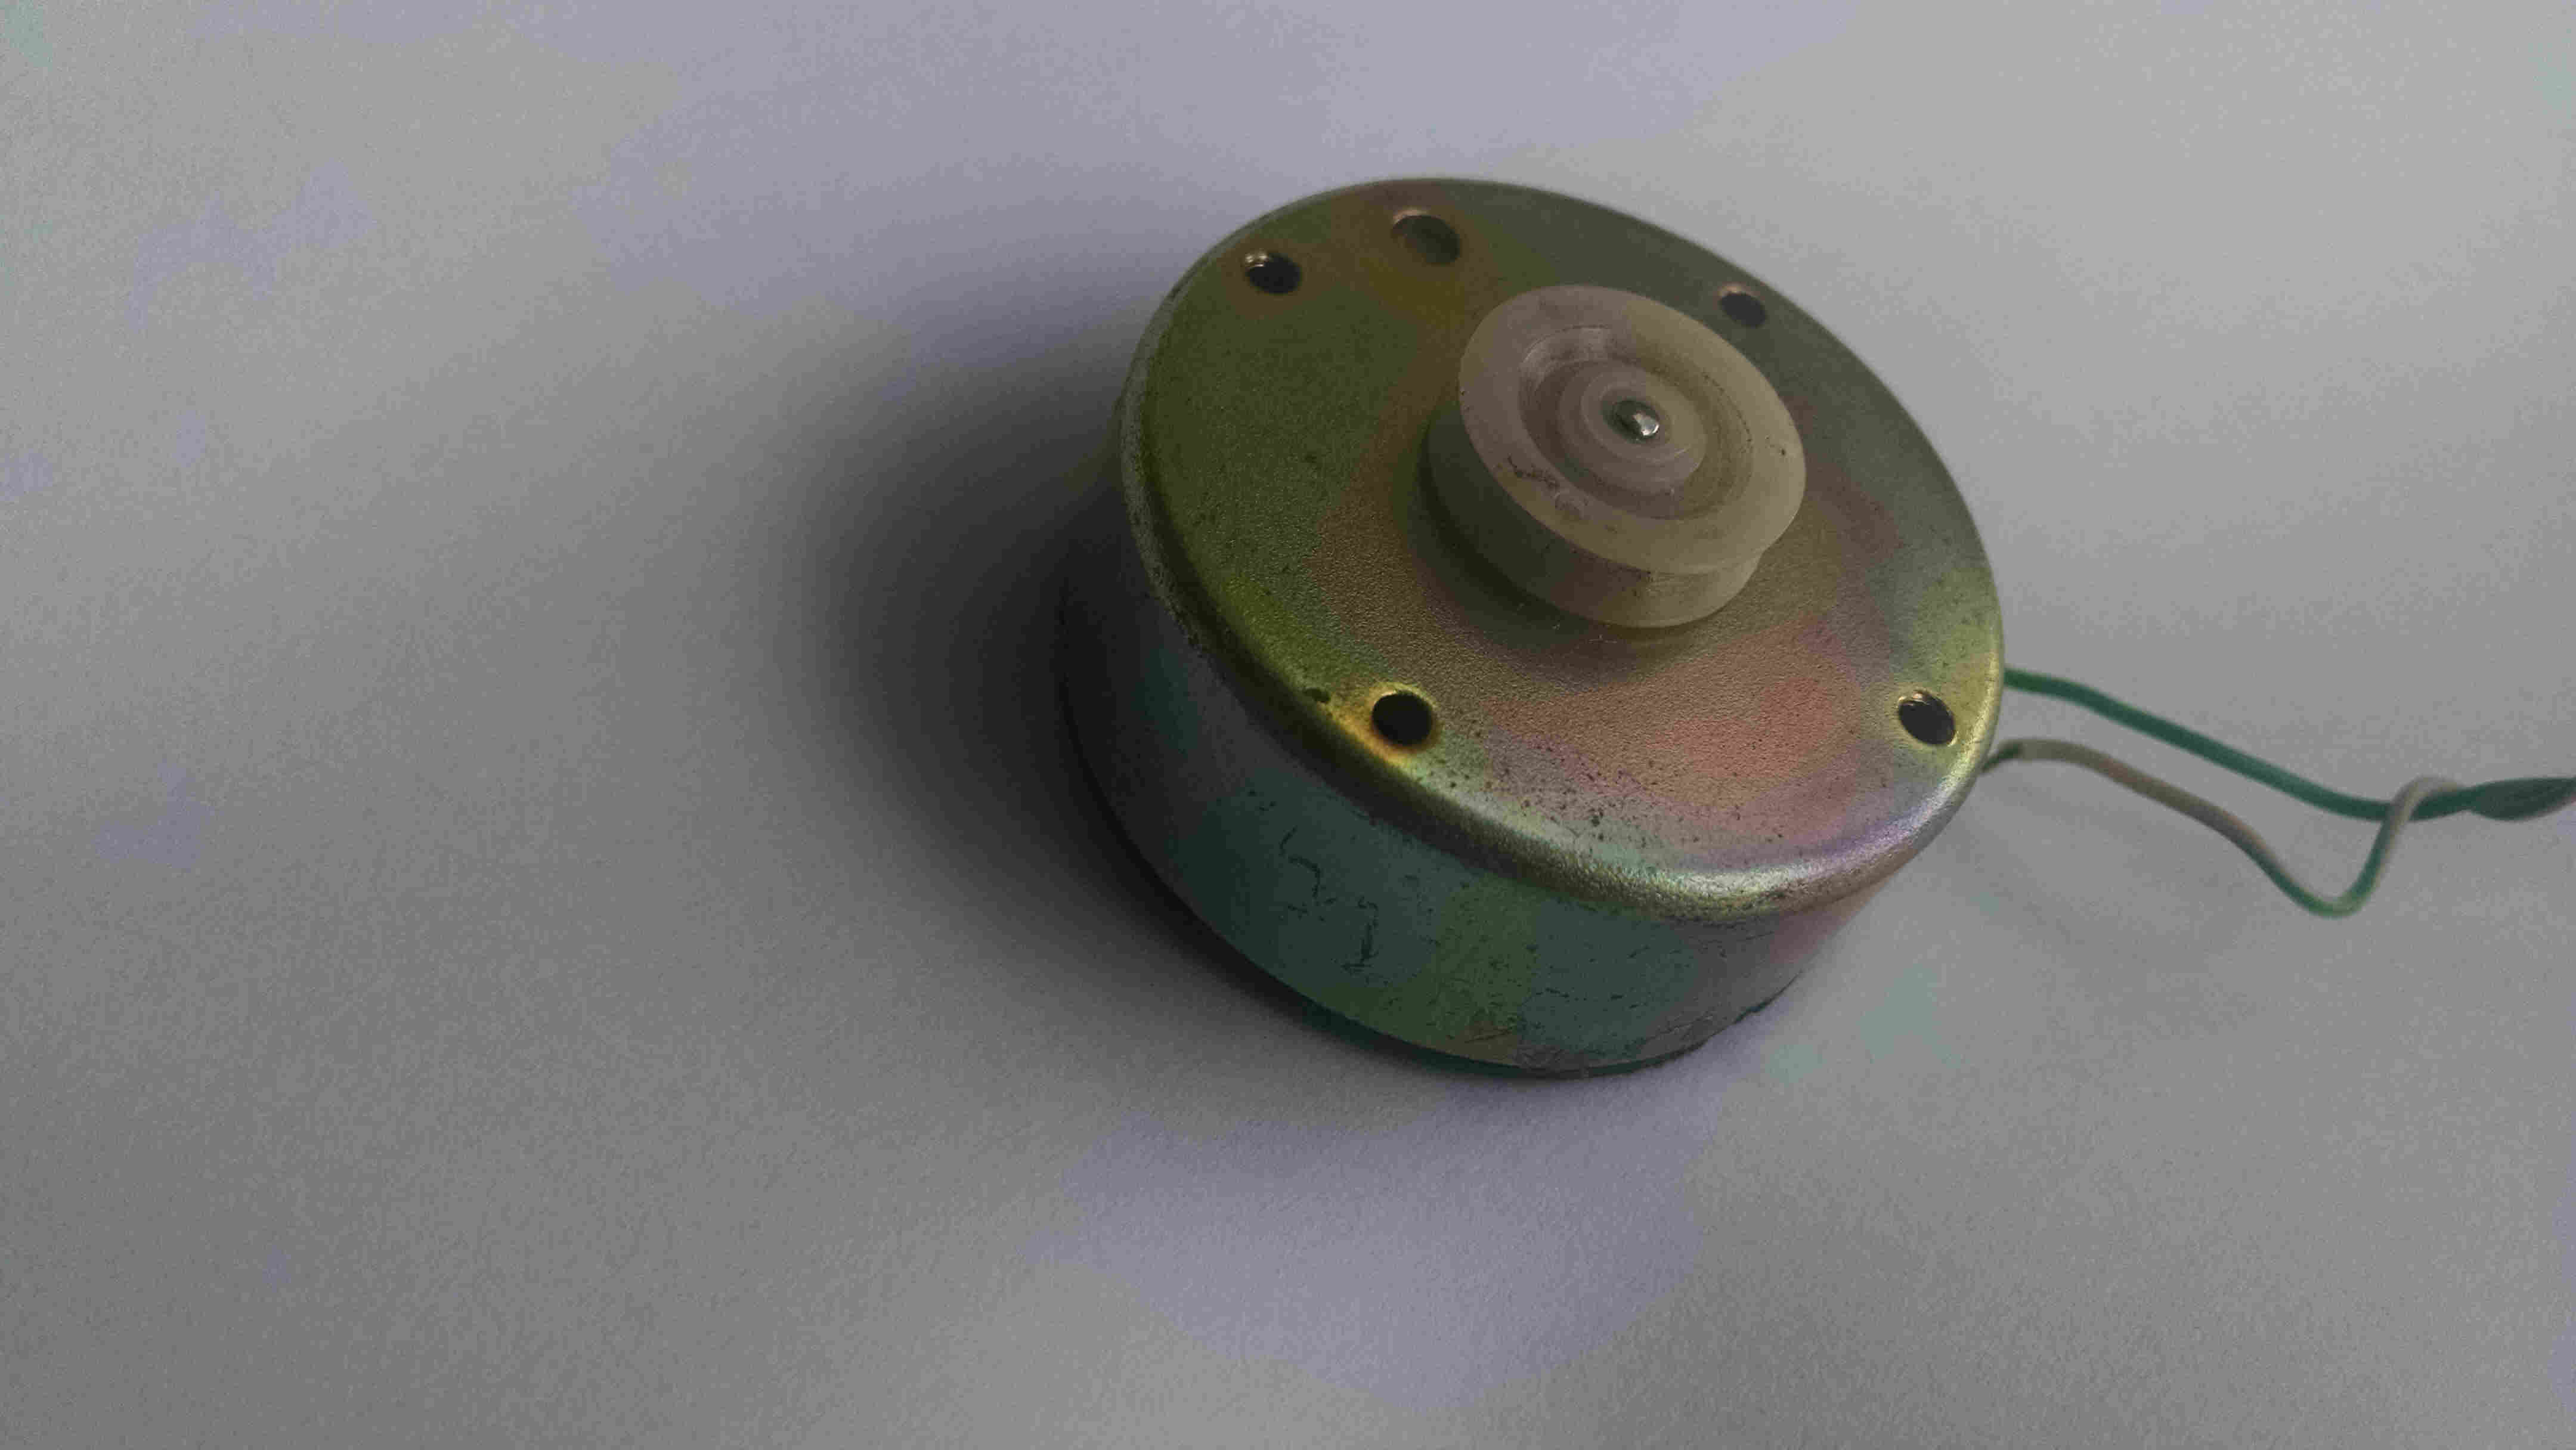
\includegraphics[scale=0.1, angle=0, clip=true, trim=1500 500 400 200]
{./imagens/motorDC.jpg}
\label{fig:motor DC}

{\small Fonte: Próprio autor}
\end{figure}

Diferente de sistemas fluídicos, as dimensões do protótipo podem ser pequenas, possibilitando uma montagem de uma pequena área em bancada e fácil transporte ou ainda comparando com sistemas térmicos, o tempo de resposta é rápida, possibilitando um tempo de testes pequeno e aquisições mais rápidas ao longo do desenvolvimento do projeto.






Para o estudo proposto foi escolhida uma placa de desenvolvimento da Texas Instruments de modelo Tiva$^{TM}$ TM4C123GH6PM, devido ao fato de que ela possui um controlador de 32bits, núcleo ARM, e permite operações utilizando ponto flutuante, entre outras características como elencadas a seguir:

\begin{itemize}
\item Núcleo (Core): ARM Cortex-M4F;
\item Performance: 80 MHz em operação;
\item Flash: 256 KB;
\item Interface de comunicação:
	\begin{itemize}
	\item  Universal Asyncrhronous Receivers/Transmitter(UART);
  	\item Inter-Integrated Circuit (I$^2$C);
	\item Universal Serial Bus (USB);
	\end{itemize}
\item Periféricos:
	\begin{itemize}
	\item General-Purpose Input/Output (GPIO);
	\item General-Purpose Timer (GPTM);
	\item Módulo PWM: Pulse Width Modulator (PWM);
	\end{itemize}
\end{itemize}

\begin{figure}[!htb]
\caption{Placa de desenvolvimento: microcontrolador com núcleo ARM-Cortex M4}
\center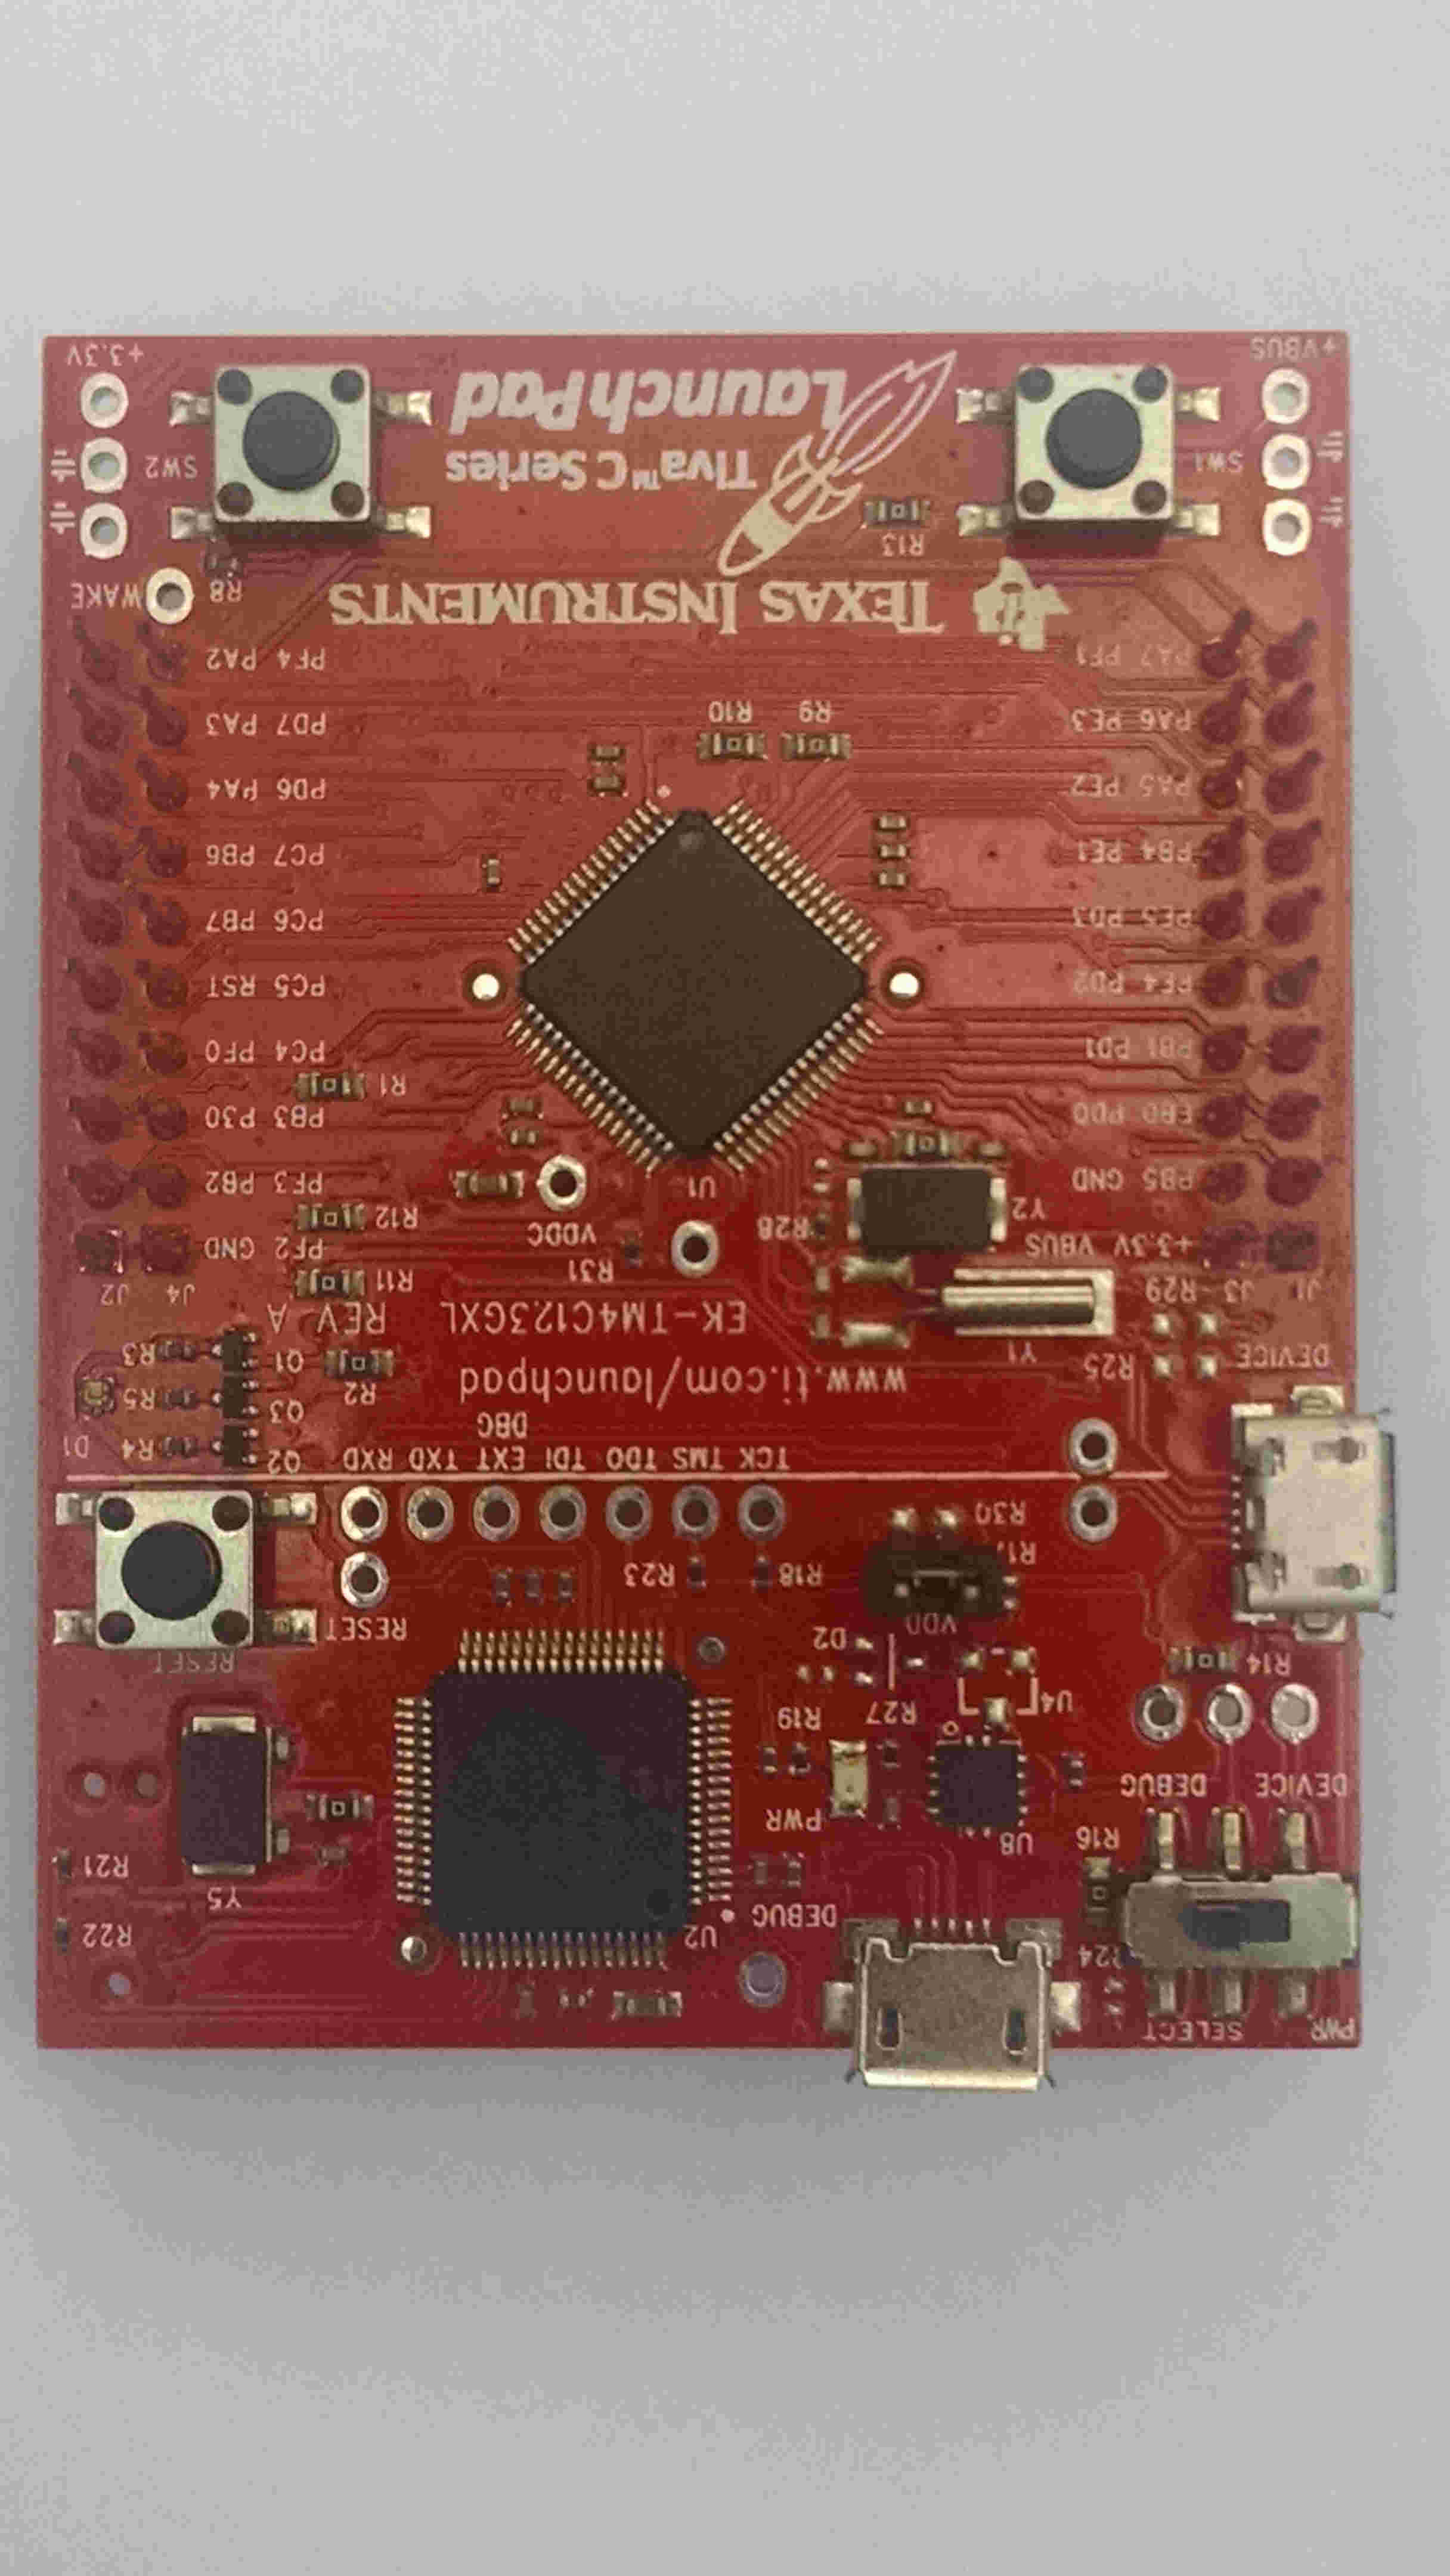
\includegraphics[scale=0.08, angle=180, clip=true, trim=0 750 60 500]{./imagens/uC-ARM.jpg}
\label{fig:uCarm}

{\small Fonte: Próprio autor}
\end{figure}

A programação do firmware, que irá embarcar o sistema de controle, será feita utilizando ferramentas em software livre, inclusive o sistema operacional GNU/Linux Debian 8, programação em linguagem C utilizando o compilador dedicado para microcontroladores de núcleo ARM, Cross GNU ARM (\texttt{arm-none-eabi-gcc}), assim como editor de texto \texttt{Vim}, terminal de comunicação \texttt{Minicom}, processador de gráficos \texttt{GNUPlot} e processaor de texto \LaTeX.








\section{ Obter um modelo do processo }
Obter a curva de comportamento do sistema para 
estabelecer a função de transferência do sistema,  
e com isso, 
estabelecer os objetivos do controle e 
identificar a variável a ser controlada.


A obtenção da curva característica se dá 
pela aquisição sucessiva do intervalo de cada rotação, 
mensurado a partir de um contador de tempo configurado adequadamente. 


O objetivo do desenvolvimento proposto, 
é realizar o controle da velocidade de rotação do disco acoplado ao eixo do motor, 
de forma a garantir que o curva característica de velocidade apresente
tempo de subida igual ou menor do que um quinto do tempo em malha aberta, 
sobressinal de no máximo 10\% e erro de regime estacionário inferior a 5\%, 
valores estes que atendem as espectativas iniciais para uma primeira implementação.


A variável controlada é a velocidade angular 
na forma de rotações por segundo (rps) 
e a variável manipilada é a tensão média 
aplicada ao motor através da técnica de 
Modulação por Largura de Pulso, 
do inglês \emph{Pulse Width Motulation - PWM}.


Assumindo que o sistema físico não tem uma aplicação crítica, 
é razoável propor um erro de 5\% para o modelo da planta, 
principalmente por se tratar de uma primeira abordagem proposta, 
sendo o intuito principal estabelecer um algorítmo ou 
modelo utilizando a LPA2v que 
atenda minimamente os requisitos de desempenho do sistema.


\section{ Estudar a LPA2v }

Baseado em trabalhos acadêmicos, artigos e livros sobre o assunto, compreender como é feita a implementação da LPA2v em tomadas de decisão contendo estados bem definidos.

\section{ Implementar um controlador utilizando LPA2v}

Implementar um controlador simples, utilizando o modelo com reticulado com subdivisões, conforme trabalhos estudados. 

Alterar a tomada de decisão do  controlador baseado em estados, por um controlador que calcula a distância entre o ponto de operação e a referência, que é a extremidade com grau de certeza máximo, e atuar sobre o sistema de forma proporcional a essa distância.


\subsection{ Estabelecer a configuração do sistema }
Estudar parâmetros necessários e limitações de configuração do controlador.

\subsection{ Descrever o controlador e parâmetros de ajuste }

Descrever em detalhes o funcionamento do controlador e estabelecer regras e sequencia de variáveis a serem parametrizadas para que o modelo do controlador possa ser reproduzido em outros momentos e situações.

\section{ Otimizar parâmetros e analisar performance }

Verificar empiricamente se os valores testados estão adequados aos requisitos de desempenho do sistema que foram previamente estabelecidos. 



